%\documentclass[ngerman,oneside]{cgsthesis}
\documentclass{cgsthesis}

\usepackage{fontspec}

% Configure Biblatex
\usepackage[defernumbers=true,natbib=true,backend=biber,
    maxbibnames=9,maxcitenames=1,style=authoryear,citestyle=authoryear,uniquelist=false]{biblatex}

% bug workaround, see http://tex.stackexchange.com/questions/311426/bibliography-error-use-of-blxbblverbaddi-doesnt-match-its-definition-ve
\makeatletter
\def\blx@maxline{77}
\makeatother

\DeclareBibliographyCategory{cited}
\DeclareBibliographyCategory{supplementary}
\AtEveryCitekey{\addtocategory{cited}{\thefield{entrykey}}}
\newcommand{\citesupplementary}[1]{\nocite{#1}\addtocategory{supplementary}{#1}}
\DefineBibliographyStrings{ngerman}{
  andothers = {\emph{et~al\adddot}}
}
\DefineBibliographyStrings{english}{
  andothers = {\emph{et~al\adddot}}
}
\addbibresource{foo-thesis.bib}
\AtEveryBibitem{\clearlist{location}}
\AtEveryBibitem{\clearfield{address}}
\AtEveryBibitem{\clearfield{doi}}

% Code listings

\usepackage{listings}
\lstloadlanguages{C++}
\usepackage{glsl}

% Thesis development


\usepackage{cgsparagraphclassification}

\usepackage[colorinlistoftodos]{todonotes}
\usepackage{outlines}
\usepackage{enumitem}
\usepackage{cleveref}
\usepackage{tabulary}
\usepackage{bm}
\setlist{itemsep=2pt,parsep=2pt}
% \setlist{topsep=0px,partopsep=0px}
% \setlist{nolistsep}

% Title page

\logo{graphics/logo_black}

\title{Design and Implementation of a Many-Light Method for Real-Time Dynamic Global Illumination}
%\subtitle{Untertitel} % z.B. englischer Titel bei Bachelorarbeit

%\subject{%
%    Bachelorarbeit\\
%    zur Erlangung des akademischen Grades\\
%    "Bachelor of Science"\\
%    (B.Sc.)\\
%    im Studiengang IT-Systems Engineering\\
%    des	 Hasso-Plattner-Instituts an der\\
%    Universit\"at Potsdam
%    \vfill
%    vorgelegt von}

\subject{%
   Masterarbeit\\
   zur Erlangung des akademischen Grades\\
   "Master of Science"\\
   (M.Sc.)\\
   im Studiengang IT-Systems Engineering\\
   des	 Hasso-Plattner-Instituts an der\\
   Universit\"at Potsdam
   \vfill
   vorgelegt von}

% \subject{%
%     Dissertation\\
%     zur Erlangung des akademischen Grades\\
%     "doctor rerum naturalium"\\
%     (Dr.\ rer.\ nat.)\\
%     in der Wissenschaftsdisziplin Informatik
%     \vfill
%     eingereicht an der\\
%     Mathematisch-Naturwissenschaftlichen Fakult\"at\\
%     der Universit\"at Potsdam\\
%     \vfill
%     von}

\author{Johannes Linke}

\publishers{%
    Aufgabenstellung und Anleitung:\\
    Prof.\ Dr.\ J\"urgen D\"ollner\\
    Daniel Limberger}

\place{Potsdam}
\date{\begin{otherlanguage}{ngerman} \today \end{otherlanguage}}


\begin{document}

\frontmatter

\maketitle

\tableofcontents

%!TEX root = foo-thesis.tex

\chapter*{Abstract}
\addcontentsline{toc}{chapter}{Abstract}

\chapter*{Zusammenfassung}
\addcontentsline{toc}{chapter}{Zusammenfassung}

\cleardoublepage


\mainmatter
%!TEX root = foo-thesis.tex

\chapter{Introduction}
\label{chap:introduction}

\todo[color=blue]{all the introduction}

\section{Problem Statement}



\section{Contribution}

single bounce only



\section{Application Areas}

Virtual city models have been done without shadows and not actually realtime: \citep{Klehm:2010:MassiveLightingCityModels}


\cleardoublepage

%!TEX root = foo-thesis.tex

\chapter{Introduction to Global Illumination and Many-Light Methods}



\todo{introduction to the various scales of GI. include \citep{jimenez:2016:AO}}

\todo{introduction to many-light methods}


\cleardoublepage

%!TEX root = foo-thesis.tex

\chapter{Concept}
\label{chap:concept}

\section{Global Illumination Pipeline Overview}
\label{sec:concept:overview}

\begin{figure}[h]
    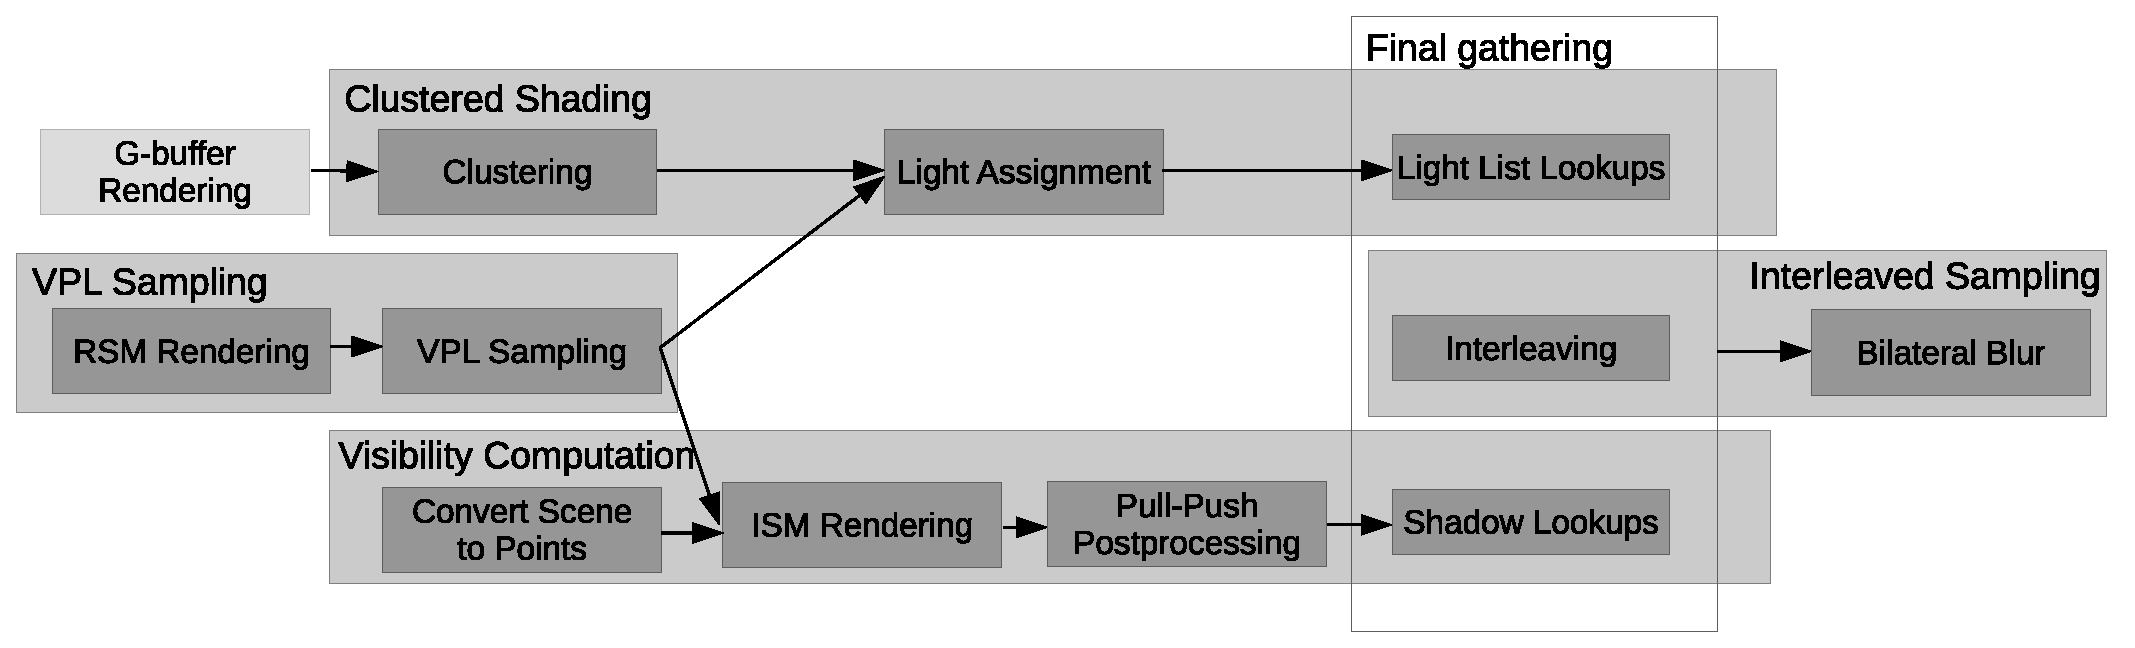
\includegraphics[width=\textwidth]{graphics/GI_pipeline_concept_rough}
    \caption{Global Illumination pipeline concept.}
    \label{fig:GIPipelineConcept}
\end{figure}


This chapter will detail the individual stages of the global illumination pipeline presented in this thesis. \Cref{fig:GIPipelineConcept} provides an overview.
Rendering the reflective shadow map and the subsequent VPL sampling (left part of middle row in the diagram) will be covered in the following section.
\Cref{sec:concept:ism} describes the rendering process for the imperfect shadow maps (lower row) in detail.
The final gathering step uses data from the clustered shading technique (upper row, detailed in \Cref{sec:concept:clusteredShading}) and performs interleaved sampling (right part of middle row, detailed in \Cref{sec:concept:interleavedSampling}).

During final gathering, clamping is used to remove singularities. Since this is a fairly trivial solution, it is not covered further.
In addition, the G-buffer rendering does not differ from common deferred rendering pipelines and is not covered further as well.


\section{Virtual Point Light Sampling with Reflective Shadow Maps}
\label{sec:concept:rsmVplSampling}

Reflective shadow maps are often preferred due to their simplicity and efficiency. Both advantages come from the fact that they are generated similar to conventional shadow maps, making them easy to implement and a perfect fit for GPUs. A downside is that they are well-suited only for computing the first light bounce.

Just like conventional shadow maps, RSMs render the scene from the viewpoint of a light. Besides the depth buffer used for shadow mapping, they render additional surface information, namely normal and color. This is similar to the additional G-buffers used by deferred rendering.

The result can be sampled to create VPLs with a certain position reconstructed from the depth buffer, and normal and color taken from the additional buffers.

VPL sampling has not been the focus of this thesis, therefore we use a rather basic approach by creating an RSM and regularly sampling it. More advanced approaches are available (see \Cref{sec:intro:relatedWorkManyLight:vplSampling}), some of which do not use RSMs (e.\,g.\ \cite{hedman2016sequential})


\section{Visibility Computation with Imperfect Shadow Maps}
\label{sec:concept:ism}

The original paper \citep{ritschel2008ism} converts the scene geometry to a point set in a preprocessing step and uses the points to efficiently render hundreds of shadow maps in parallel. They use splatting to render the points and fill the resulting holes in the shadow maps with a simplified version of the pull-push algorithm presented in \citep{Marroquim:2007:reconstruction}.

\citet{ritschel2011ismsViewAdaptive} build on this by converting the scene to a triangle texture dynamically, and sampling the points from that texture. Instead of computing a triangle texture, \citet{barak2013temporally} use the tessellation units of recent GPUs to dynamically convert triangles into points.
We follow this approach since it is relatively straightforward to implement and inherently dynamic, but have not implemented the adaptive sampling from \citet{ritschel2011ismsViewAdaptive} yet.
\citet{ritschel2008ism} also present multi-bounce indirect illumination with their technique, which we have not implemented.

In contrast to \citet{ritschel2008ism}, we have found the pull-push postprocessing to be of little benefit when using regular point splatting. Instead, we propose to render the points as single pixels, which opens interesting optimization opportunities, but in turn requires the pull-push algorithm to reconstruct the scene surfaces.

The following subsections describe the regular point splat rendering process and subsequently detail the pull-push algorithm that is used when rendering single-pixel points.


\subsection{Point Rendering with Splatting}

To convert the scene into points, all its triangles are first tessellated to meet a certain maximum size in order for the point conversion to not introduce extreme inaccuracies. Of the smaller tessellated triangles, the center and area are calculated and a point with matching center and area is created. While it might be more performant to create points just on the vertices of the triangles, at the same time it will be more inaccurate since this approach will enlarge the rendered area considerably over the triangle's extents.

Now a random VPL is chosen per point and backface culling is performed. Likewise, points that lie behind their VPL's illuminated hemisphere are culled before splatting the point into the respective ISM. For performance reasons, a simple paraboloid projection is used for the ISMs in lieu of conventional cubemaps. Here, another advantage of using points comes into play: Compared to triangles, it is trivial to perform a paraboloid projection on them.

As an optimization, we iterate over several VPLs per point, collect those that pass the culling test and render to all the collected ones. More on this in \cref{chap:implementation}.

To remove holes in the resulting shadow map, the original paper implements a simplified variant of \citet{Marroquim:2007:reconstruction} that only uses depth information from the point rendering. We found that this approach has little benefit over simply enlarging all the point splats during rendering, therefore we did not use it when using splat rendering.



\subsection{Point Rendering with Pull-Push Postprocessing}

As an alternative to point splat rendering, this subsection proposes a second approach that follows the algorithm of \citet{Marroquim:2007:reconstruction} more closely with the intent to obtain higher-quality shadow maps. More specifically, the points are rendered as a single pixel, albeit with additional attributes like size and normal. These are then used in a subsequent reconstruction pass to create an (ideally) hole-free shadow map. This approach also allows a point to be rendered into multiple shadow maps with a moderate performance impact, more on this in \Cref{sec:impl:singlePixelRendering}.

To provide a rough overview, the pull-push algorithm proposed by \citet{Marroquim:2007:reconstruction} is a ``pyramid-method'' (see \cite{Strengert:2006:Pyramid}) that uses the mipmap levels of a texture to first condense and then spread the data in the texture, in this case the sparse point set representing the scene. During the pull phase, it aggregates the information from four pixels of a finer level to one pixel of a coarser level. The subsequent push phase aggregates four pixels of a coarser level to one pixel of a finer level, but only if the pixel of the finer level contains no data or is determined to belong to an occluded surface. This way, closed surfaces are derived from single-pixel points.

\subsubsection{Pull Phase}
The pull phase reads four pixels of a finer level, computes an aggregate representation of them and writes the result to one pixel of the next coarser level. However, it only considers pixels that pass the following tests: First, they need to contain a valid depth at all (i.\,e., a point must have been rendered into this pixel) and second, the point in this pixel must not be occluded. A point is considered to be occluded if it is outside the depth interval of the frontmost of the four pixels used for interpolation.

Figuratively speaking, the depth interval of a point denotes the range in which other points are considered to belong to the same surface and can be used for interpolation. For the rendered points, the depth interval is simply $[d;d+k]$ where $d$ is the points depth and $k$ an arbitrarily chosen constant. For interpolated points, the new depth interval spans the interpolated depth of the point to the highest depth value of the depth intervals of all ``parent'' points.

To calculate the attributes for a new point, the depth and radius of the parent points are interpolated in between with equal weights. Since the center of the aggregated point might not match with the position of the pixel (this happens if not all four pixels are used for interpolation), a displacement vector is also calculated and stored to accurately describe the point's location.


\subsubsection{Push Phase}

Analogous to the pull phase, the push phase reads four pixels of the coarser level, rejects pixels that do not pass certain tests, and writes one output pixel into the finer level. First, just like in the pull phase, the input pixels must contain a valid depth and not be occluded to be considered. Additionally, a radius check is performed: If the pixel's location is outside the point's extents described by the displacement vector and its radius, then the point is not considered either. This is done to limit a point's influence to its actual size.

The target output location in the finer level might already contain data computed during the pull phase. This data is overwritten if its depth is behind the interpolated point's depth interval, i.\,e., if the original data is considered to be occluded. Otherwise, the original point is left untouched, as it is likely more accurate than the just computed, interpolated point.

Since the input and output pixel's location do not match the way they do during the pull phase, the weights used for interpolation during the push phase are not uniform, see Figure~\ref{fig:???}.

\todo{some figure about weights during pull-push}

 \citet{Marroquim:2007:reconstruction} also use the point's normals to correctly limit the point's size, and \citet{Marroquim:2008:reconstruction2} propose Gaussian weights based on the pixel's distance to the point's location, instead of constant weights solely based on pixel locations. Both of these additions we have not implemented yet.



\section{Clustered Deferred Shading}
\label{sec:concept:clusteredShading}

In real-time graphics applications, primarily video games, a technique called \textit{clustered shading} \citep{olsson2012clustered}, has seen increased usage. Its goal is to increase the efficiency of lighting a scene with multiple light sources.
The effectiveness of clustered shading in the context of many-light global illumination has not been studied so far to our knowledge, and we aim to contribute a few data points to this end.

The clustered shading technique works as follows: First, the view frustum is divided into a fixed number of three-dimensional clusters. For each fragment, the respective cluster is determined with the purpose to ignore all clusters with no fragments in them. Then, for each cluster, all lights (in this case, VPLs) whose illuminated region is intersected by the cluster are added into a light list for that cluster. All other lights are ``culled'', i.\,e.\ not added to the list.

When shading a fragment, the algorithm first determines the fragment's cluster again, and then iterates only over the lights in that cluster's light list. This way, all the lights that have been discarded in the previous step do not need to be considered per fragment.

This technique yields the most gains when using lights with a limited radius. In that case, the culling is all the more effective since all lights that are farther away from a cluster than the light's radius can be culled as well. However, many-light methods often use infinite radii to enable light transport over long distances. Nonetheless, one can still expect to cull roughly half of all lights with this technique in a many-light context.

As an extension, \citet{olsson2012clustered} propose to calculate explicit bounds for the fragment's position in each cluster to enable more precise culling. We expected only moderate performance gains from that and have not implemented it.

Another extension is to use the surface normal's direction as fourth dimension after the three spatial dimensions for clustering, allowing for a kind of backface culling for even greater efficiency. While this seems more promising in terms of performance gains, we have not implemented it yet either.


Clustered shading is an extension and improvement to \textit{tiled shading} \citep{Olsson:2011:TiledShading}, which uses screen-space tiles instead of view-space clusters. Tiled shading has previously been combined with many-light global illumination by \citet{Tokuyoshi:2016:Stochastic}. They use an order of magnitude more lights than we do, but stochastically limit them in range. As a result, the light culling is much more effective in their case.
We implemented tiled shading as well and will compare it to clustered shading in \Cref{sec:results:clusteredShading}.


\section{Interleaved Sampling}
\label{sec:concept:interleavedSampling}
Interleaved sampling \citep{Keller:2001:InterleavedSampling} is often used to tremendously improve the performance of GI methods with a negligible quality impact.

The general idea is as follows: Instead of calculating all samples per pixels, the samples are distributed over a block of pixels. Now, since each pixel has only a partition of the samples, there is obviously information missing per pixel. Visually, this becomes apparent in the form of structured noise. To this end, a geometry-aware blur similar to \citet{laine2007incremental} is used to spread the information and thereby even out the noise. The blur is often implemented in a separated fashion, although it is, strictly speaking, not a separable one due to its geometry-awareness.

Since adjacent pixels now access disjoint sets of samples, naive implementations of this technique usually show bad cache coherence. To improve on this, \citet{segovia2006non} proposed ``de-interleaving'' to group and process those pixel simultaneously that use the same sample set.

Effectively, when applied to blocks of $n^2$ pixels, this technique cuts down the cost of sampling to $ 1 / n^2 $ at the expense of smoothing high-frequency changes in the samples over $n$ pixels. Since global illumination is usually of low frequency, i.\,e.\ adjacent pixels usually receive a similar amount of indirect light, interleaved shading does not significantly affect quality when applied to global illumination. However, it falls short near depth and normal discontinuities, where the geometry-aware blur ignores several pixels. Nevertheless, even in this case the quality degradation is hardly noticeable as soon as the global illumination results are blended over the rendered image, see \Cref{sec:results:interleavedShading}.

In most aspects we follow the standard approach for interleaved shading. The only notable deviation is the implementation of de-interleaving that does not use any separate splitting and merging passes. For details, see \Cref{sec:impl:interleavedShading}.

%!TEX root = foo-thesis.tex


\chapter{Implementation}

\section{Used Libraries and the Framework gloperate}

\todo[color=green]{software architecture?}

- some architecture diagram of dependencies?
- gloperate as framework
    - uses qt
- libzeug provides GUI elements
- globjects as an object-oriented abstraction over OpenGL
- glbinding provides OpenGL bindings, directly called sometimes
- GLM provides math and easier interaction with the OpenGL API
- no further relevance for this thesis:
    - assimp for model loading
    - glkernel provides kernels for our SSAO implementation
    - cpplocate ???

\section{Rendering Pipeline Overview}
- would be much the same as the concept pipeline...
- show what's compute shader and what not?
- it's basically lighting plus
    - g-buffer generation
    - shadowmap which is part of the RSM,
    - SSAO
    - deferredshading
    - srgb and HDR.
    - all of this is not
- model loading?
- kernel generation?


\section{RSM Generation and VPL Sampling}
\label{sec:impl:rsmAndVplSampling}
- use the exact same code for RSM generation as for G-Buffer generation
- re-use RSM as shadowmap
    - usually, one might want to decouple this since they likely need different resolutions/cascading schemes etc. One could also render the RSM with a less detailed version of the scene. Since we had no culling and LOD implemented, we were bottlenecked on geometry complexity and chose to do this in one pass.
    - we use variance shadowmapping. so we add the variance buffer if we're rendering an RSM, and disable another buffer (non-face normals).

- with a compute shader, we sample the RSM in a regular pattern and write VPLs into a buffer
- VPLs are position, normal, color
- we prepare a second buffer with a single vec4 with position in the first three values and normal packed into the last value.
- we do that since the ISM rendering (Section~\ref{sec:impl:ismRendering}) and light list calculation (Section~\ref{sec:impl:clusteredShading}) do not need color and especially ISM rendering reads several VPLs per point, using a lot of bandwidth.
- Because of the regular sampling, the noise produced during interleaved shading (Section~\ref{sec:impl:interleavedShading} or only results? there was a paper that sorts VPLs to avoid the noise...) is more structured. To help with that, we permutate the VPL order with a random permutation computed on CPU

\section{ISM Rendering}
\label{sec:impl:ismRendering}
- Our ISM rendering normally draws all the geometry in the scene.
- In the tessellation control shader, the tesselation levels are determined depending on the triangle size.
- The tessellation evaluation shader does nothing besides correctly interpolating the triangle's vertices.
- The geometry shader, which now recieves a small (tesselated) triangle, computes the point data
- i.e. position: center of triangle, radius: distance of center to farthest triangle vertex, normal: the face normal taken from the original, non-tessellated triangle.

- the geometry shader then calculates a random VPL ID. We used the point's position to seed the random number generator. This makes the ISMs temporally unstable when the geometry moves, but we couldn't find a stable seed.

\todo[color=blue]{implement randomness based on barycentric coordinates}

- two approaches:

- either the geometry shader itself reads the VPL with the index it determined, projects the point according to the VPL's data, sets gl\_PointSize to the projected size, and emits a vertex.
- also, output mode is points.

- \citet{Marroquim:2007:reconstruction} actually works with single-pixel ``splats''. since in this case we're not depending on the hardware rasterizer for good performance, this inspired the following approach:

- instead of splatting, the geometry shader puts points into buffer
- one buffer per VPL for stability
- buffers index marks the first VPL to try
- then, per point in each buffer, starting with the respective VPL, we test a fixed number of VPLs (e.\,g. 16) and collect up to 4 that pass culling tests.
- specifically, backface culling and points that are located behind the VPL, i.\,e. not in the hemisphere pointing along the VPL's normal.
- we then render the point as a single pixel into the 4 collected VPLs.

\todo{part of this into concept}


- hole mitigation
- when splatting, the quality difference improvement achieved with an additional pull-push algorithm compared to slightly larger splats seemed not worth the performance impact, therefore we chose to simply enlarge all splats a bit.
- when using compute shaders, we need pull-push by design.

\todo{explain pullpush implementation}

\section{Interleaved Shading with Compute Shaders}
\label{sec:impl:interleavedShading}
- often, this technique is implemented by splitting the G-buffer into several smaller G-buffers, each containing all pixels with the same sample set \cite{segovia2006non}, a process called de-interleaving. Each G-buffer is processed with it's respective sample set, and then the buffers are re-interleaved into a large G-Buffer again.

- instead we do something crappy and want to improve on it...
- we chose 4x4
\todo[color=blue]{implement no scattered reads. maybe packed G-buffers for that? maybe better normal packing for that?}

- Since only a subset of all samples is processed per pixel and this subset repeats every four pixels, this process results in structured noise (see Figure \ref{fig:???})
- therefore, geometry-aware blur similar to \citet{laine2007incremental}. doesn't smooth over edges. See code snippet \ref{listing:???}. every pixel has all the information now ideally.
- VPL shuffling helps a great deal!

\section{Clustered Deferred Shading}
\label{sec:impl:clusteredShading}

%!TEX root = foo-thesis.tex


\chapter{Results and Discussion}
\label{chap:results}

This chapter details the performance and rendering quality characteristics of the implemented techniques and examines their memory usage. For each technique, it will subsequently discuss the up- and downsides.

\section{Scenes, Settings and Testing System}
\label{sec:results:settings}

The implementation is tested in the Crytek Sponza and San Miguel scene, with 260k and 7.9M triangles respectively, both provided by \citet{McGuire2011Data}. Unless otherwise noted, the parameters used for the measurements and screenshots are:

\begin{outline}
    \1 1920x1080\,px output resolution
    \1 1024 VPLs
    \1 2048²\,px ISM texture, i.\,e., 64²\,px per ISM
    \1 Single-pixel point renderer enabled, 16 VPLs considered per point, up to 4 collected
    \1 4x4 interleaving pattern
    \1 Tiled shading enabled
\end{outline}

\noindent
The hardware specification of the testing system is as follows:

\begin{outline}
    \1 Intel Xeon W3530 with four cores at 2.8\,Ghz
    \1 NVIDIA GeForce GTX 980 factory-overclocked by ca. 4\%, driver version 375.57
\end{outline}

The GTX 980 has been locked to its base clock rate of 1164\,Mhz using SetStablePowerState.exe\footnote{\url{https://developer.nvidia.com/setstablepowerstateexe-\%20disabling\%20-gpu-boost-windows-10-getting-more-deterministic-timestamp-queries}}, preventing its GPU Boost feature\footnote{\url{http://www.geforce.com/hardware/technology/gpu-boost-2}} from altering the results depending on the GPUs temperature and power draw. This comes at the cost of preventing the GPU from using its maximum potential, but combined with the factory-overclocking, the results should be close to the real-world performance.

\pagebreak


\section{Rendering Time Breakdown}
\label{sec:results:RenderingTimeBreakdown}


\begin{table}[h]
    \centering
    \captionabove{Timing breakdown of an entire frame rendered by the presented software. Timings are in milliseconds.}
    \begin{tabulary}{0.98\textwidth}{| L | L | L | L | L | L | L || L |}
        \hline
        G-Buffer & RSM & ISM & GI & SSAO & Combine & Blit & Total \\ \hline
        0.6\,ms & 0.2\,ms & 2.7\,ms & 3.2\,ms & 1.4\,ms & 0.3\,ms & 0.3\,ms & 8.70\,ms \\
        \hline
    \end{tabulary}
    \label{tab:results:timing_breakdown_frame}
\end{table}

\Cref{tab:results:timing_breakdown_frame} gives an overview of the time needed for rendering a single frame. The Crytek Sponza scene and default settings have been used. All timings measure GPU time only; there are no noteworthy calculations done on the CPU. With a total of 8.7\,ms, the application achieves real-time framerates while leaving room for more expensive calculations, higher output resolutions, or more detailed scenes.

The GI, SSAO, and combine pass operate in screen space and are mostly dependent on the screen size (and, of course, on light and sample count in the case of GI and SSAO, respectively). The G-Buffer and RSM generation follow the usual performance characteristics and are mainly dependent on output resolution and geometric complexity. The performance behavior of the ISM rendering heavily depends on the settings and is further detailed below. The blit phase copies a texture to the back buffer and serves debugging purposes only.


\section{RSM Generation and VPL Sampling}
\label{sec:results:RsmAndVplSampling}

\begin{figure}[htb]
    \centering
    \begin{subfigure}[b]{1.0\textwidth}
        \centering
        \includegraphics[width=1.0\linewidth]{screenshots/RSM_diffuse}%
        \caption{}
    \end{subfigure}\\
    \par\medskip
    \begin{subfigure}[b]{0.49\textwidth}
        \centering
        \includegraphics[width=1.0\linewidth]{screenshots/RSM_normal}%
        \caption{}
    \end{subfigure}%
    \hfill
    \begin{subfigure}[b]{0.49\textwidth}
        \centering
        \includegraphics[width=1.0\linewidth]{screenshots/RSM_depth}%
        \caption{}
    \end{subfigure}%
    \caption{A reflective shadow map, with its (a) diffuse, (b) normal, and (c) depth buffer.}
    \label{fig:results:RSMBuffers}%
\end{figure}%


As explained before, the RSM generation re-uses most of the code of the G-Buffer generation; see \Cref{fig:results:RSMBuffers} for an impression on the rendered result. Accordingly, the performance characteristics are similar to the regular geometry pass of deferred renderers.

Since the implemented VPL sampling distributes the samples over the entire shadow map, we simply limited the VPLs' locations to the relevant area by tuning the light's extents. As a result, an aspect ratio chosen specifically for each test scene is used. Since our implementation re-uses the RSM as shadow map for direct lighting, we chose a resolution of 512²\,px (or, in the case of the Sponza scene, 1024x256\,px), which is more than required by the naive VPL sampling. The RSM is rendered in 0.17\,ms for the Sponza scene.

The VPL sampling itself takes only several microseconds and is negligible. Bear in mind that, in order to achieve high quality levels, a more elaborate sampling algorithm needs to be implemented, which can in fact take most of the available time. For instance, the implemented sampling does not take the relevance of the sampled VPLs to the current frame into account. This causes the entire system to be rather inefficient because it chooses lights that might contribute little or nothing to the rendered output (\Cref{fig:results:RSMUnfavorable}. An additional downside of the naive sampling is the poor temporal stability when the scene light moves. This is due to each VPL staying at the exact same position in the light's viewport, so their positions strictly follow the light's movement, jumping over depth discontinuities along the way.

\begin{figure}[htb]
\centering
  \begin{tabular}{@{}c@{}}
    \includegraphics[width=1.0\textwidth]{screenshots/RSM_unfavorable} \\
  \end{tabular}
  \caption{A visualization of inefficiently placed VPLs. Each of the brigth spots is a VPL. Here, they are all placed on the roof pointing upwards. Since there is no further geometry above them that could be illuminated, they do not contribute to the final image.}
  \label{fig:results:RSMUnfavorable}
\end{figure}




\section{ISM Rendering}
\label{sec:results:ism}

This section presents the results for visibility testing using imperfect shadow maps. The next three subsections will show the outcome in terms of quality, performance, and memory usage. The technique does not handle high geometric complexity of the test scenes well; this is detailed in the fourth subsection. Afterwards, the two different ISM renderers are compared and the suitability of ISMs for global illumination in general is discussed.


\subsection{Quality}
\label{sec:results:ism:quality}

\begin{figure}[htb]
\centering
  \begin{tabular}{@{}cc@{}}
    \includegraphics[width=.48\textwidth]{screenshots/ism_splat_cropped} &
    \includegraphics[width=.48\textwidth]{screenshots/ism_single_pixel_cropped}
  \end{tabular}
  \caption{ISMs rendered using the splat renderer (left) and single-pixel renderer (right) with default settings. The single-pixel renderer performs interpolation between points, renders more points, and does not let points bleed into neighboring ISMs, but takes more time.}
  \label{fig:results:isms}
\end{figure}

\Cref{fig:results:isms} shows a few ISMs rendered with the splat and single-pixel renderer. The imperfections do show, and not only through the low resolutions. The distortion of the surface silhouettes by the splat renderer or postprocessing contribute their part, making it hard to identify which part of the Crytek Sponza is rendered. However, keep in mind that the imperfections, while being noticeable in each individual ISM, are expected to partly cancel each other out and result in an acceptable average error in the final rendering.

\begin{figure}[htb]
\centering
  \begin{tabular}{@{}cc@{}}
    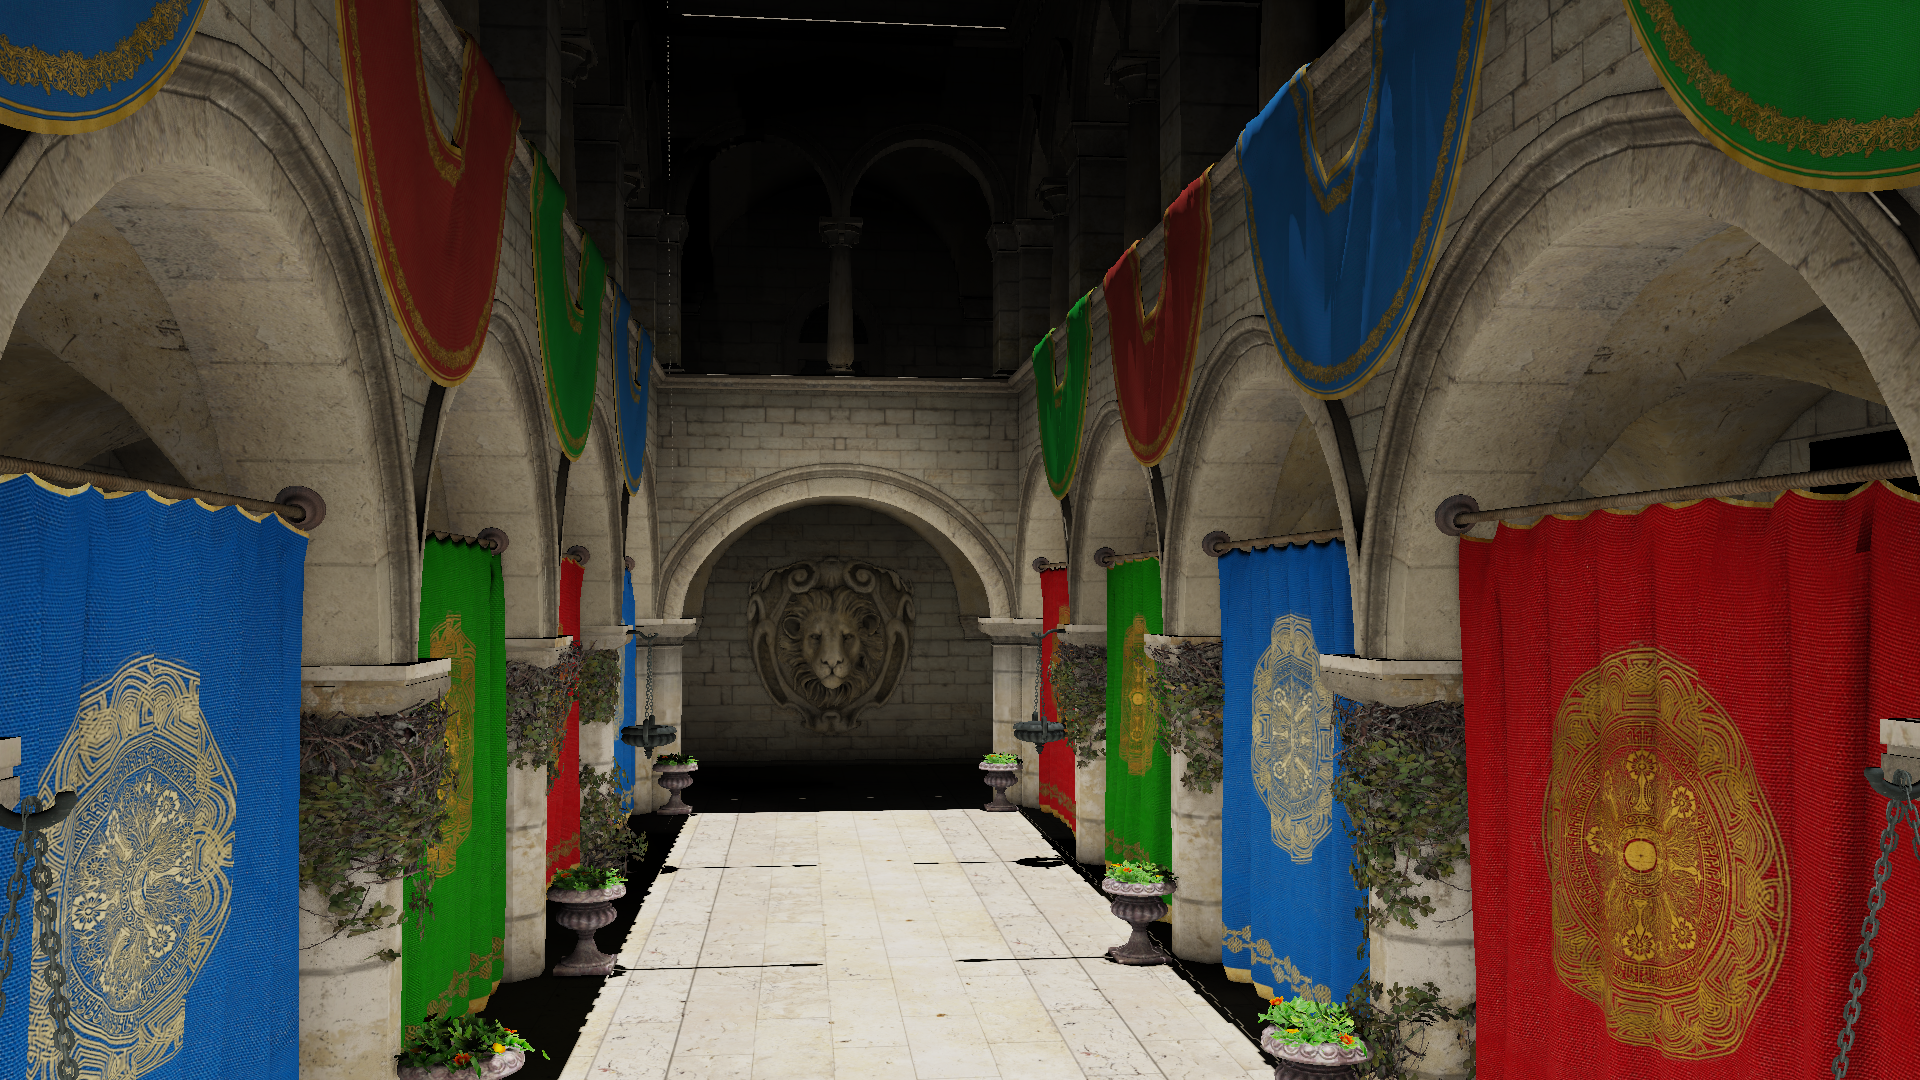
\includegraphics[width=.48\textwidth]{screenshots/darkening_splat} &
    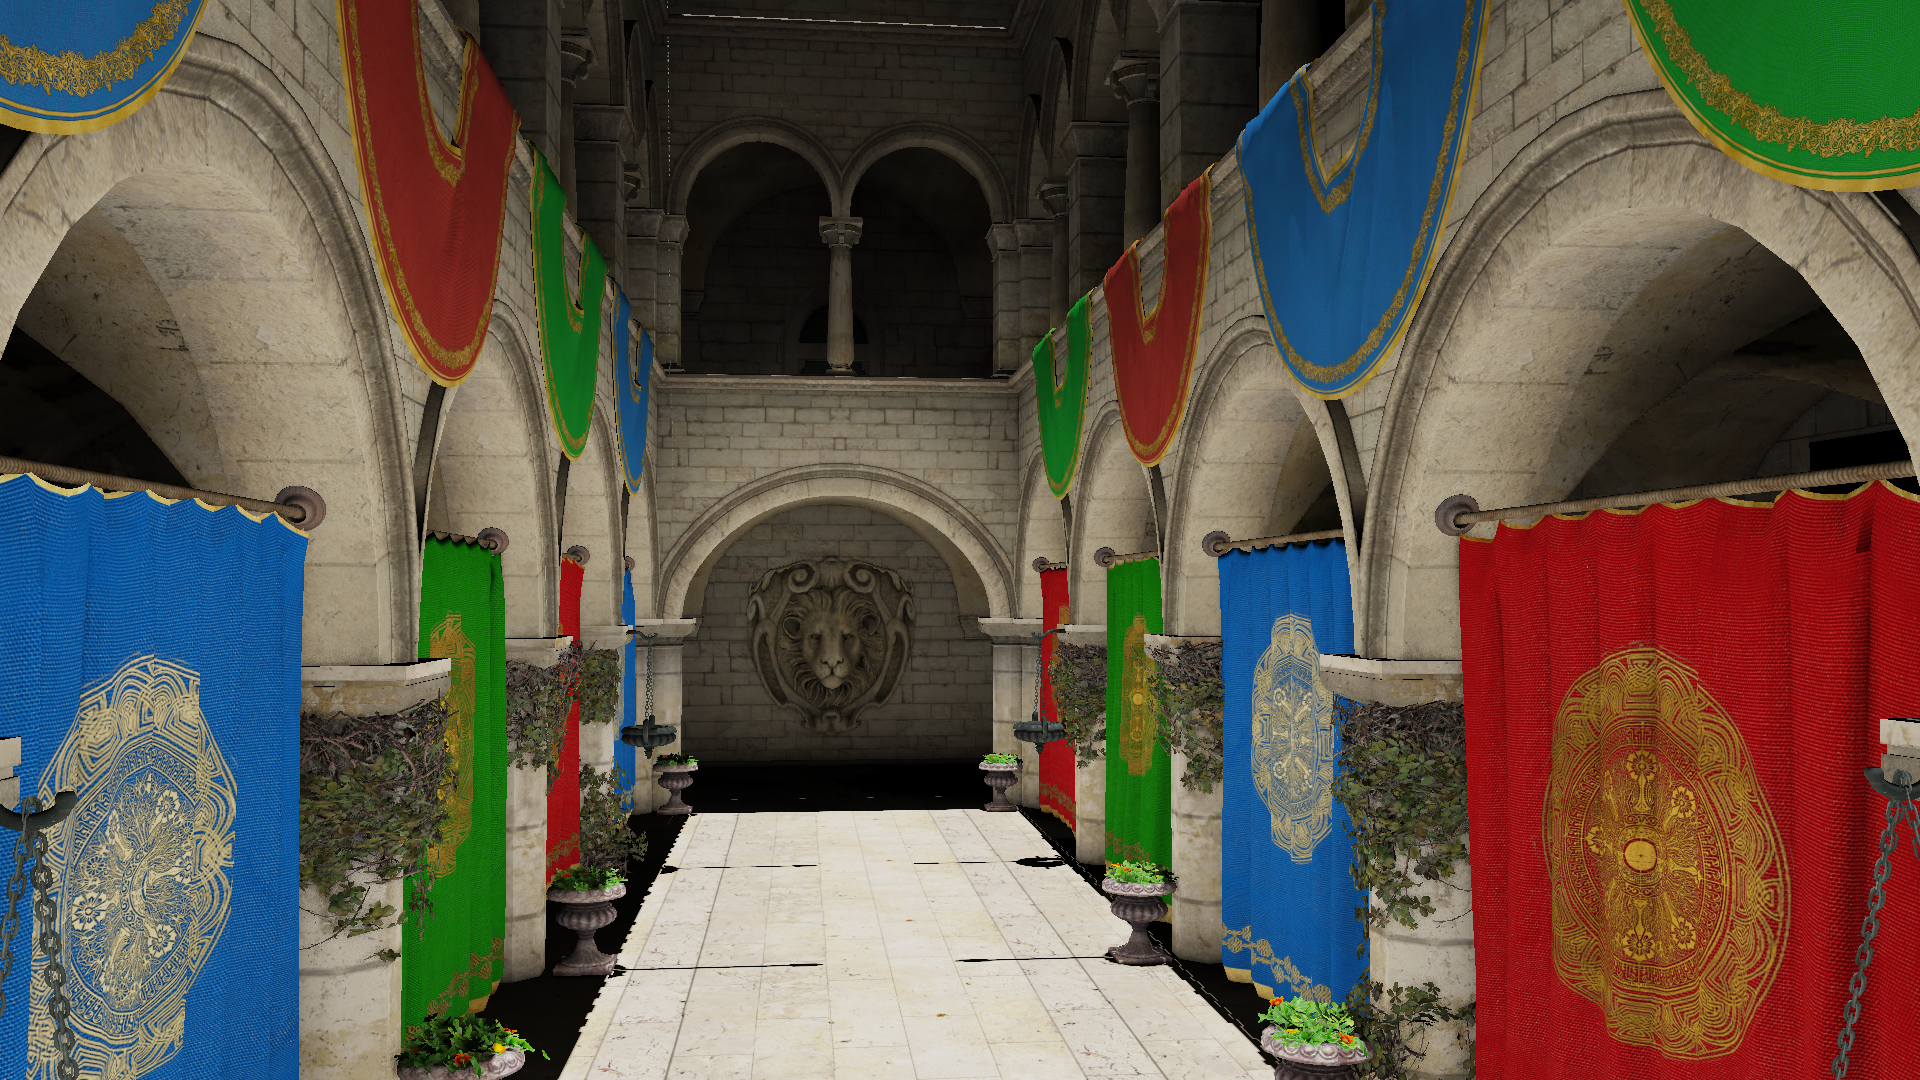
\includegraphics[width=.48\textwidth]{screenshots/darkening_single_pixel}
  \end{tabular}
  \caption{Darkening caused by the splat renderer (left) compared to the single-pixel renderer (right). Note that there is no skylight rendered, which leads to an unnaturally dark upper part in the image even for the single-pixel renderer.}
  \label{fig:results:ismDarkening}
\end{figure}

Comparing the screenshots in \cref{fig:results:ismDarkening}, it becomes apparent that the splat renderer causes visible darkening in the upper part of the image. The reason is probably that the point splats are always oriented towards the camera and do not take the point's normal into account when rendering, amplifying the usual aliasing artifacts of common shadow maps. As a result, any point size larger than one pixel causes surfaces that are not directly facing the camera to appear nearer than they actually are when doing shadow lookups in ISMs. A larger shadow bias could compensate for that but would introduce heavier light leaking. Another possibility is to use the normal to calculate a point's depth per fragment at a potentially high performance cost.

As the single-pixel renderer does not use splats, this problem is largely mitigated. In a certain way it performs the per-fragment depth calculation implicitly during interpolation in the postprocessing phase.


\begin{figure}[htb]
\centering
  \begin{tabular}{@{}cc@{}}
    \includegraphics[width=.48\textwidth]{screenshots/leaks_splat} &
    \includegraphics[width=.48\textwidth]{screenshots/leaks_single_pixel}\\
    \includegraphics[width=.48\textwidth]{screenshots/leaks_splat_exposure} &
    \includegraphics[width=.48\textwidth]{screenshots/leaks_single_pixel_exposure}
  \end{tabular}
  \caption{Light leaks caused by imperfect shadow maps rendered with the splat renderer (left) and single-pixel renderer (right). VPLs from beneath the curtains leak light onto the wall and ceiling, while VPLs on the pillars and curtains light the floor. The renderings in the bottom row were rendered with a higher exposure for illustration. }
  \label{fig:results:leaks}
\end{figure}


\Cref{fig:results:leaks} shows a case which the ISM technique has difficulties with. The image should be mostly dark or at least uniformly lit through the small gap below the curtains, instead the wall and ceiling appear too bright and the floor displays several artifacts. The root cause is that the VPLs are placed right behind the curtains, so the occluding geometry, i.\,e., the curtain, is very near to the light source. Due to the randomness involved when selecting point sets for rendering ISMs, it often happens that the points near to the light source are rendered into other ISMs, leaving a large hole behind. The single-pixel renderer fares a bit better than the splat renderer since it uses more points, but does not provide a satisfactory result either.



\begin{figure}[htb]
\centering
  \begin{tabular}{@{}cc@{}}
    \includegraphics[width=.48\textwidth]{screenshots/bias_splat} &
    \includegraphics[width=.48\textwidth]{screenshots/bias_single_pixel}\\
      \includegraphics[width=.48\textwidth]{screenshots/bias_splat_exposure} &
      \includegraphics[width=.48\textwidth]{screenshots/bias_single_pixel_exposure}
  \end{tabular}
  \caption{Light leaks caused by using a relatively large shadow bias with the purpose to hide artifacts of the ISMs. The screenshots to the left use the splat renderer, the right ones the single-pixel renderer. The bottom row was rendered with a higher exposure.}
  \label{fig:results:bias}
\end{figure}

Our implementation hides some of the inaccuracies of ISMs by using a relatively large shadow bias. The resulting light leaks are shown in \Cref{fig:results:bias}. While the splat renderer fares better here, it does so mainly by darkening the whole image since it uses rather large points. The single-pixel renderer on the other hand correctly lets light illuminate the left wall through the columns, but shows a rather noisy result.




\subsection{Performance}
\label{sec:results:ism:performance}

\begin{table}[h]
    \centering
    \captionabove{Timings of the ISM renderers with different settings.}
    \begin{tabulary}{0.98\textwidth}{| L | L | L | L |}
        \hline
        Splat Default Settings & Single-Pixel Default Settings & Splat with Single-Pixel Settings & Single-Pixel with Splat Settings \\ \hline
        1.08\,ms & 2.74\,ms & 10.14\,ms & 2.31\,ms \\
        \hline
    \end{tabulary}
    \label{tab:results:ism_timings}
\end{table}

\Cref{tab:results:ism_timings} shows the time needed for rendering the ISMs with both renderers and different settings. Note that the comparison between the two renderers with default settings is not a fair one, since the single-pixel renderer renders more points and by default clamps each point's extents to its ISM. If the splat renderer is changed to behave similarly, it takes 0.3 additional milliseconds for clamping, and 8.66 additional milliseconds for using the same technique to collect VPLs that the single-pixel renderer uses.

There are several reasons for this heavy slowdown: First, this is implemented by emitting multiple vertices in the geometry shader, which is known to have poor performance on current GPUs. Second, the additional fillrate and overdraw became an issue when rendering too many points, a bottleneck that is unlikely to occur when using the single-pixel renderer. And third, while the single-pixel renderer uses shared memory to load the 16 VPLs once, the geometry shader of the splat renderer has no access to shared memory and has to load all 16 VPLs per invocation, creating high register pressure.

Conversely, if the single-pixel renderer does not perform clamping, the push phase needs 0.07\,ms less (0.85\,ms to 0.78\,ms), and when it considers only one VPL per point, the point renderer takes 0.41\,ms less (0.65\,ms to 0.24\,ms).

Since the presented implementation uses no adaptivity, these numbers are independent from the viewport. They are however slightly affected by VPL placement, since it influences culling. In a second scenario, where the sunlight shines directly from above, all VPLs are placed on the floor facing up. As a result, much fewer points are culled during ISM rendering, resulting in slightly higher timings. Both renderers need about 0.1\,ms more in this case.


\subsubsection{Detailed Performance Measurements for the Single-Pixel Point Renderer}
\label{sec:results:ism:performanceSinglePixelRenderer}


\begin{table}[h]
    \centering
    \captionabove{Timing breakdown of the single-pixel point renderer.}
    \begin{tabulary}{0.98\textwidth}{| L | L | L | L || L |}
        \hline
        Point Collection & Point Rendering & Pull Phase & Push Phase & Total\\ \hline
        0.83\,ms & 0.65\,ms & 0.39\,ms & 0.85\,ms & 2.72\,ms\\
        \hline
    \end{tabulary}
    \label{tab:results:timing_breakdown_single_pixel}
\end{table}

\begin{table}[h]
    \centering
    \captionabove{Timing breakdown of the pull (PL) and push (PS) phase. The numbers of the individual steps indicate to which mipmap level they write, which is why the pull phase starts at 1 and the push phase has descending numbers. All timings are in milliseconds.}
    \begin{tabulary}{0.98\textwidth}{| L | L | L | L | L | L | L | L || L | L || L |}
        \hline
        PL 1 & PL 2 & PL 3 & PL > 3 & PS > 2 & PS 2 & PS 1 & PS 0 & PL Total & PS Total & Total \\ \hline
        0.16 & 0.16 & 0.04 & 0.03   & 0.06   & 0.08 & 0.30 & 0.41 & 0.39     & 0.85     & 1.24\\
        \hline
    \end{tabulary}
    \label{tab:results:timing_breakdown_pull_push}
\end{table}


\Cref{tab:results:timing_breakdown_single_pixel} gives more detailed performance measurements of the single-pixel renderer, while \cref{tab:results:timing_breakdown_pull_push} further breaks down the individual steps of the pull and push phase. Note how the timings scale roughly as expected (PL 3 and PS 2 are taking roughly four times longer than PL 2 and PS 1, respectively), except for the first and last step. This is due to the reduced input data size (or output size, respectively), as explained in \cref{sec:impl:pullPushPostprocessing}. Also note how the push phase does take roughly the time of the pull phase if it were not for the last phase, where it writes to the full 2048²\,px of miplevel zero, whereas the largest miplevel written to by the pull phase is level one with 1024²\,px.



\subsection{Memory Usage}
\label{sec:results:ism:memory}

The point splat renderer requires no more memory than the ISM texture itself requires, which is 8\,MB for a 2048²\,px 16-bit depth buffer. The single-pixel renderer requires additional memory. First, it uses a buffer for storing the points. This is implemented as four-channel 32-bit float texture, with the first three channels containing the position, and the last channel containing radius (8 bit) and normal (24 bit, see \cite{Cigolle:2014:NormalPacking}). With a maximum point count of 2048 per ISM (keep in mind they are rendered into multiple ISMs later), this buffer uses 32\,MB.
The additional textures created are the render target of the single-pixel renderer (single-channel 2048x2048\,px, 32-bit integer, 16\,MB), the mipmap levels used by the pull-push algorithm (four channels, 32-bit, approx. 22\,MB) and the final ISM (same format as used by the splat renderer, 8MB).

Added together, the single-pixel renderer requires a total of 79\,MB. There remains some rooms for optimization: For instance, one channel of the mipmap levels is unused (OpenGL does not offer three-channel images), and for some textures, using 16-bit floats instead of 32-bit float might be sufficient.


\subsection{Problems with High Geometric Density}
\label{sec:results:ism:densityProblems}

A more demanding test case is the San Miguel scene with 7.9M triangles. The most apparent problem of the presented implementation is the lack of adaptivity to the current viewport in addition to the lack of LOD methods. As a result, all 7.9M triangles are used every frame to render the ISMs, with corresponding performance results: The point collection phase of the single-pixel renderer now takes 12.0\,ms, while the point rendering takes an additional 5.3\,ms. The time needed by the postprocessing is unchanged since it works on fixed resolution textures. The splat renderer takes 12.0\,ms, which is the exact same amount of time as the point collection phase of the single-pixel renderer, even though the latter has no rasterization to perform. This demonstrates how this process is bottlenecked by geometric complexity.


\begin{figure}[htb]
\centering
  \begin{tabular}{@{}c@{}}
    \includegraphics[width=1.0\textwidth]{screenshots/san_miguel_wide} \\
  \end{tabular}
  \caption{A rendering of the San Miguel scene in the presented implementation. Note the unnaturally dark region behind the pillars.}
  \label{fig:results:san_miguel_wide}
\end{figure}

\begin{figure}[htb]
\centering
  \begin{tabular}{@{}cc@{}}
    \includegraphics[width=.48\textwidth]{screenshots/san_miguel_ugly_shadow} &
    \includegraphics[width=.48\textwidth]{screenshots/san_miguel_ugly_shadow_gi_only}
  \end{tabular}
  \caption{A particularly inaccurate shadow produced by ISMs. The right image shows only indirect light. Ideally, the shadow would be much smoother. The low-frequency noise is caused by choosing random points per ISM, while the many edges of the shadows are caused by the basic shadow mapping algorithm, which performs a simple binary choice.}
  \label{fig:results:san_miguel_ugly_shadow}
\end{figure}

\Cref{fig:results:san_miguel_wide} shows an example screenshot of the San Miguel scene. There are several factors contributing to an overly dark region behind the pillars. First, during ISM rendering all points are rendered into at least one pixel, which makes them take out too much light if they are actually smaller than one pixel. This is especially the case with the thin structures of the chairs and trees. Additionally, the implementation simulates only one bounce, making it impossible for the floor behind the pillars to be lit at all. Another problem case is shown by \Cref{fig:results:san_miguel_ugly_shadow}, where the table and chairs cast a visibly inaccurate shadow.


\subsection{Comparison of the Splat and Single-Pixel Renderer}
\label{sec:results:ism:comparison}

The single-pixel renderer provides numerous advantages over the splat renderer: Using a compute shader to render points lifts the restrictions of the fixed-function pipeline and, e.\,g., allows rendering each point into multiple ISMs without large performance losses. Quality-wise, it can reproduce surfaces more accurately by correctly interpolating between points.

The drawbacks obviously include the additional rendering time and memory. Besides, the added complexity should not be underestimated. Specifically, we found it hard to fine-tune the pull-push algorithm to produce satisfactory results, especially in the face of the low resolutions of ISMs and the limited data available for reconstruction after selecting a random and sparse set of points.



\subsection{Discussion}
\label{sec:results:ism:discussion}

Imperfect shadow maps have several deficits, some of which are inherent to the technique and difficult to solve, while others are specific to the implementation choices and tradeoffs in the presented implementation and might be easier to overcome.

First, ISMs reduce the scene's geometry to points. At the resolution that is achievable in a real-time budget, this is already a rough approximation that loses a lot of accuracy.

Second, because a sparse set of points is used for each ISM, each point must be enlarged to accommodate for the neighboring points that are likely missing in the chosen ISM. For instance, if an area is represented by a thousand points and only one tenth of all points is used for each ISM, each remaining point's area must be enlarged by a factor of ten to result in an equally large area in the rendered output. Of course, this approach leads to deformed geometry since points at the edges of the area are enlarged as well, growing over the borders of the original geometry.

Third, ISMs also have numerical issues. For instance, both the splatting and postprocessing approaches ignore the distortion caused by the paraboloid projection, and thus might render even simple surfaces incorrectly. This contributes to the necessity of using a relatively large shadow bias. At the cost of additional complexity, this can likely be solved with relative ease.

Fourth, and this is in our view the most important shortcoming, ISMs handle geometry in the vicinity to VPLs badly (\Cref{fig:results:leaks}). To sufficiently approximate such surfaces when rendering ISMs, one would need to greatly increase the number of points created near VPLs, possibly in addition to stepping away from using a fully random approach for point selection, and one would have to select a specific point set for each ISM depending on the VPLs location.

As for most global illumination algorithms, a massive improvement would be to differentiate between large-scale scene geometry that is important for diffuse light bounces, and smaller geometry of lesser importance. While the latter can possibly be ignored altogether with only minor losses in quality, the shape of large-scale geometry is all the more important to preserve (relatively) precisely.

The San Miguel scene is a good example for this: While the small detail work like dishes and small plants make up most of the geometry and thus most of the rendering time, they contribute only very little to global illumination. This is where the presented implementation suffers most from the lack of level-of-detail methods.



\section{Interleaved Sampling using Compute Shaders}
\label{sec:results:interleavedShading}

Interleaved sampling substantially reduces the number of lights that are processed per pixel. Using a 4x4 interleaving pattern, each pixel processes only a sixteenth of all lights, ideally speeding up the final gathering phase by a factor of 16. However, an additional blur pass is required to mask the noise that results from interleaving, which takes additional time.


\begin{table}[h]
    \centering
    \captionabove{Timings of interleaved sampling (IS) with a block size of 4x4. Note that the blur pass is mandatory when using interleaved sampling; the middle column merely illustrates the efficiency of the presented implementation, while the last column shows the practical speedup that is achieved.}
    \begin{tabulary}{0.98\textwidth}{| L | L | L | L | L |}
        \hline
        Without IS & With IS & Speedup & Blur Pass & Speedup with Blur\\ \hline
        40.24\,ms & 2.61\,ms & 15.42 & 0.63\,ms & 12.42\\
        \hline
    \end{tabulary}
    \label{tab:results:timings_interleaved_shading}
\end{table}



\begin{figure}[htb]
    \centering
    \begin{subfigure}[b]{0.20\textwidth}
        \centering
        \includegraphics[width=.95\textwidth]{screenshots/interleaved_before}
        \caption{}
        \label{fig:results:interleaved_before}%
    \end{subfigure}%
    \begin{subfigure}[b]{0.20\textwidth}
        \centering
        \includegraphics[width=.95\textwidth]{screenshots/interleaved_horizontal_blur}%
        \caption{}
        \label{fig:results:interleaved_horizontal_blur}%
    \end{subfigure}%
    \begin{subfigure}[b]{0.20\textwidth}
        \centering
        \includegraphics[width=.95\textwidth]{screenshots/interleaved_final}%
        \caption{}
        \label{fig:results:interleaved_final}%
    \end{subfigure}%
    \begin{subfigure}[b]{0.20\textwidth}
        \centering
        \includegraphics[width=.95\textwidth]{screenshots/interleaved_without}%
        \caption{}
        \label{fig:results:interleaved_without}%
    \end{subfigure}%
    \begin{subfigure}[b]{0.20\textwidth}
        \centering
        \includegraphics[width=.95\textwidth]{screenshots/interleaved_difference_gi}%
        \caption{}
        \label{fig:results:interleaved_difference_gi}%
    \end{subfigure}\\
    \par\medskip
    \begin{subfigure}[b]{0.333\textwidth}
        \centering
        \includegraphics[width=.95\textwidth]{screenshots/interleaved_without_textured}%
        \caption{}
        \label{fig:results:interleaved_without_textured}%
    \end{subfigure}%
    \begin{subfigure}[b]{0.333\textwidth}
        \centering
        \includegraphics[width=.95\textwidth]{screenshots/interleaved_with_textured}%
        \caption{}
        \label{fig:results:interleaved_with_textured}%
    \end{subfigure}%
    \begin{subfigure}[b]{0.333\textwidth}
        \centering
        \includegraphics[width=.95\textwidth]{screenshots/interleaved_difference_shaded}%
        \caption{}
        \label{fig:results:interleaved_difference_shaded}%
    \end{subfigure}%

      \caption{Interleaved sampling results. The top row shows indirect light only. From left to right: (a) Result of the final gathering phase without the bilateral blur, (b) with the horizontal phase of the blur applied, (c) with both phases applied, (d) result of the final gathering phase without using interleaved sampling, (e) difference between (c) and (d). Bottom row: (f) final result after blending when using interleaved sampling, (g) whithout interleaved sampling, (h) difference between (f) and (g). Difference values are multiplied by eight.}
      \label{fig:results:interleaved_quality}
\end{figure}


\Cref{tab:results:timings_interleaved_shading} shows timings of the presented implementation. Most notably, the interleaved sampling technique introduces very little overhead, as indicated by the speedup of 15.42 compared to the theoretical maximum of 16. In absolute terms, a speedup of 16 would require the final gathering phase to take 2.51\,ms. As a result, the technique introduces 0.1\,ms of overhead.

When considering the blur phase, the overhead adds up to 0.73\,ms and the speedup is lowered to 12.42. Of course this is still a substantial improvement, especially considering the negligible quality impact.

This technique requires an additional buffer for storing the intermediate result of the blur phase, while the final result can be written into the same texture that was used for final gathering. The texture format \texttt{GL\_R11F\_G11F\_B10F} is used here, resulting in roughly 2\,MB additional storage at full HD. The presented implementation does not re-use the final gathering texture to keep the results of all stages available for debugging purposes.


\subsubsection{Discussion}
Interleaved sampling is an obvious win for many-light global illumination methods. Paying the full cost of evaluating all VPLs per shading point is simply unnecessary due to the low-frequency nature of global illumination. Adapting the shading frequency to a similarly low level is the only reasonable choice for real-time applications.

In fact, given the unnoticable quality impact (\Cref{fig:results:interleaved_quality}) of interleaved sampling when using a 4x4 block size, larger block sizes, e.\,g., 8x8 as used by \citet{hedman2016sequential} should be considered. Especially with the advent of high-resolution displays, lowering the shading frequency of global illumination effect even further might be necessary to keep the costs down to a reasonable level. However, the performance gains from lower sample counts will be offset in part by larger blur radii that come with larger block sizes.

Going further, this technique is limited by how well the blur phase is able to mask the noise in more difficult areas with lots of depth discontinuities like vegetation. To this end, one option might be to collect fragments that receive too few information during shading and blurring, and re-process them with larger sets of VPLs in a second pass (similar to \cite{Lauritzen:2010:Deferred}). Temporal reprojection methods \citep{Jimenez:2016:FilmicSMAA} that re-use information from previous frames and use different sets of VPLs per frame would be another natural extension of interleaved sampling.



\section{Clustered and Tiled Deferred Shading}
\label{sec:results:clusteredShading}

Clustered deferred shading and tiled deferred shading reduce the number of light calculation operations by clustering fragments and culling lights against those clusters. As such, if implemented correctly, they do not affect quality at all, but are purely performance optimizations.

\begin{table}[h]
    \centering
    \captionabove{Timings of the final gathering stage without optimizations, with clustered shading (CS) and with tiled shading (TS). Each line is a different camera position. Note that the timing ``With CS'' includes roughly 0.06\,ms for the clustering phase and 0.13\,ms for the light list phase.}
    \begin{tabulary}{0.98\textwidth}{| L | L | L | L | L |}
        \hline
        Scene & Without CS/TS & With CS & With TS \\ \hline
        Sponza 1 & 3.41\,ms & 2.80\,ms & 2.40\\
        Sponza 2 & 3.94\,ms & 3.63\,ms & 3.09\\
        Sponza 3 & 2.68\,ms & 1.64\,ms & 1.34\\
        San Miguel & 4.75\,ms & 5.21\,ms & 4.43\\
        \hline
    \end{tabulary}
    \label{tab:results:timings_clustered_shading}
\end{table}

As visible in \Cref{tab:results:timings_clustered_shading}, both clustered shading and tiled deferred shading can improve the performance of the final gathering phase considerably: In one of the measurements 50\,\% of the computation time is saved with tiled shading.


It is interesting that clustered shading, being the successor of tiled shading, performs noticeably worse in the context of many-light methods. This is true even for the San Miguel scene, in which the higher amount of depth discontinuities should be favorable to clustered shading. While these performance characteristics might be specific to the presented implementation, there are plausible reasons that they might apply generally: Due to the infinite light radii used, the percentage of culled lights is generally low. Therefore it might be the better choice to optimize for the worst case and implement a low overhead solution like tiled shading, instead of a more accurate solution like clustered shading that might improve the culling rate, but comes with more overhead.

An impression of the amount of overhead introduced by clustered shading is given by the San Miguel scene, from which the last line of measurements is taken. This scene runs much slower even when only considering the final gathering phase, because most VPLs are placed on the walls and floor, pointing inwards or upwards respectively. Therefore much of the geometry lies on the illuminated side of most VPLs, resulting in very little performance gains from culling.

With a low culling rate, clustered shading actually slows down the final gathering phase by 0.46\,ms. While 0.19\,ms of these are fixed costs added by the clustering and light list calculation phases, the final gathering shader was slowed down by 0.27\,ms as well. This might be caused by the indirection when accessing lights, since instead of reading from the light buffer directly, the light list with indices is accessed first before reading the light buffer with a dynamic index. Another explanation might be the divergent data flow, since threads from the same work group can access different light lists and thus different light data and shadow maps, possibly hurting cache efficiency.

As discussed in section \Cref{sec:impl:clusteredShading}, clustered shading consumes about 2\,MB of memory. The tiled shading algorithm however, being integrated into the final gathering shader, uses no additional VRAM at all.

\subsubsection{Discussion}

The presented measurements make tiled shading seem like a clear winner, but as so often the situation is more complicated. The integration of tiled shading into the final gathering shader, while an efficient and easy to implement solution, is inherently less flexible than clustered shading. For instance, \citet{olsson2012clustered} propose to use normals as another dimension besides the three spatial ones, further improving culling efficiency. While this is presumably easy to integrate into the more flexible approach taken with clustered shading, the integrated tiled shading is constrained by the amount of available shared memory, which makes it challenging to take additional dimensions into account.

%!TEX root = foo-thesis.tex


\chapter{Conclusion and Future Work}
\label{chap:conclusion}

In this thesis we have presented a rendering system that simulates global illumination at real-time framerates. It takes only a few milliseconds for computing indirect lighting, making it suitable for use in real-time applications on today's hardware.

In addition to imperfect shadow maps rendered with splatting, a second renderer based on compute shaders has been implemented. With the flexibility provided by compute shaders, it is able to render a high amount of points more efficiently compared to the splat renderer, which relies on geometry shaders. Extended with a high-quality postprocessing, it renders shadow maps of noticeable higher quality than the splat renderer, but the resulting quality is limited by the input data, a randomly selected and sparse set of points representing the scene. Several  failure cases have been identified where the presented implementation generates artifacts clearly visible even to the untrained eye.

Interleaved shading has traditionally been performed by the means of several shader passes, which split a buffer into several smaller ones, perform processing on them, and merge these buffers again. This thesis has presented an implementation that is integrated into the final gathering shader, making splitting and merging buffers obsolete while still processing the workload cache-coherently. Its near-perfect efficiency, ease of implementation, and the fact that it requires no additional memory make this implementation the obvious choice when compute shaders are available on the given platform.

Two light culling techniques well-known in the video games industry, tiled and clustered deferred shading, have been applied to many-light global illumination. While tiled deferred shading's simplicity allowed for a compact implementation integrated into the final gathering shader, clustered deferred shading promised higher culling efficiency at the expense of higher overhead. The results have shown this overhead to be not worth the gains, making clustered deferred shading not the perfect candidate for light culling in a global illumination context using many-light methods. There are extensions, however, that could improve its culling efficiency to the point where it causes no slowdown in the worst case. Tiled deferred shading, on the other hand, is a clear performance win and again, rather easy to implement, but limited in its maximum culling efficiency.


Looking forward, going beyond random point sampling for creating imperfect shadow maps is desirable, since the randomness is limiting their quality. The implementation of more advanced surface reconstruction techniques, starting with the full extent of the algorithm presented by \citet{Marroquim:2007:reconstruction}, would likely further enhance the ISM's quality.

Given how common the usage of interleaved sampling is, it is surprising that little work has been done to maximize the technique's impact. For instance, thoroughly investigating the correlation between performance and quality when changing the block size would give implementers a guideline on which block sizes to choose in which scenarios.

There is still potential in the clustered deferred shading technique, for instance by using surface normals for more efficient culling. Mipmapping the ISMs and using them for culling, performing an early shadow lookup for entire clusters of fragments, would be interesting as well.

However, the final gathering phase is quite fast at least on high-end hardware, and, more importantly,  not detrimental to quality. While rendering the ISMs is fast as well, their quality is lacking and limiting the potential use of the presented technique. Improving their precision by, for example, improving the point sampling or surface reconstruction or investigating triangle-based approaches, is in our view the path with the largest potential benefit.


\chapter{Todos}

\subsubsection{figures}

\todo[inline]{Pipeline figures for all sections in implementation. e.g. create RSM, which is then sampled, and the samples are put into two buffers.}

\todo[inline]{Interleaved shading algorithm figure comparing buffer splitting vs compute shaders in addition to pipeline figure \Cref{sec:impl:interleavedShading}}

\todo[inline]{Temporal coherence/frame-to-frame diff when light moves figure. end of \Cref{sec:results:RsmAndVplSampling}}

\todo[inline]{culling efficiency visualization}


\subsubsection{content}

\todo[inline]{some closing remarks. add some personal evaluations, broad statement about complexity}

\todo[inline]{Lui: summaries at the end of chapters}

\todo[inline,color=yellow]{implement some moving object. show temporal coherency when it moves. or even moving spherical light. \Cref{sec:results:ism}}

\todo[inline]{put VPL shuffling comparison anywhere, maybe results \Cref{sec:results:ism:quality}}


\subsubsection{misc}

\todo[inline]{repository readme}


\todo[inline]{brighter version for print}
\todo[inline]{noindent after figures}
\todo[inline]{latex warnings}
\todo[inline]{orphans and widows, also single words on a line}


% \include{chap-examples}
% \include{chap-moreexamples}

% force line breaks inside URLs
\begingroup
\setcounter{biburllcpenalty}{7000}
\setcounter{biburlucpenalty}{8000}
\sloppy

\printbibliography[title={Bibliography},category=cited,heading=bibintoc]
\endgroup

% Further Reading
% \citesupplementary{Alvarez.etal-1992}
% \printbibliography[title={Weiterf{"u}hrende Literatur},category=supplementary,resetnumbers=true,heading=bibintoc]

% Debug: uncited
\nocite{*}
\printbibliography[title={Uncited},notcategory=cited,resetnumbers=true,heading=bibintoc]

\appendix
% \include{appn1}

\backmatter

%!TEX root = foo-thesis.tex

\pagestyle{plain}

\chapter*{Eidesstattliche Erklärung}

Ich erkläre hiermit an Eides statt, dass ich die vorliegende
Arbeit ohne unzulässige Hilfe Dritter und ohne Benutzung anderer
als der angegebenen Hilfsmittel angefertigt habe; die aus anderen
Quellen direkt oder indirekt übernommenen Daten und Konzepte sind
unter Angabe des Literaturzitats gekennzeichnet.
Diese Arbeit hat in gleicher oder ähnlicher Form noch keiner Prüfungsbehörde vorgelegen.

\vspace{1.5cm}

\noindent
\begin{tabular}{p{0.4\linewidth}p{0.1\linewidth}p{0.4\linewidth}}
Potsdam, \today &&\\
\cline{1-1}
\cline{3-3}
(Ort, Datum)&&(Unterschrift)
\end{tabular}


\end{document}
